\chapter{Programación de Placas Gráficas}

\section{Introducci\'on}
La constante demanda de capacidad en las aplicaciones gr\'aficas, motivada sobre todo por el auge de los videojuegos y las películas de animación, han provocado que el poder de cómputo de las unidades de hardware paralelo haya sufrido una marcada evoluci\'on desde su aparici\'on.
Dicha evoluci\'on ha tenido como consecuencia la rivalizaci\'on y posterior superaci\'on por parte de las GPUs al poder de procesamiento con el que cuentan las CPUs tradicionales \cite{Harris06}.
En la siguiente sección se resume la historia de la programación de las placas gráficas, desde las primeras placas configurables, las cuales sólo permitían controlar superficialmente su comportamiento, hasta las placas que permiten una programación de propósito general sobre ellas.

\section{Historia del Shader Programable}
Las placas gráficas o GPUs son microprocesadores, y por lo tanto tienen su propio lenguaje assembler, el cual puede programarse para realizar una tarea específica.
A diferencia de las CPUs, las GPUs no son herramientas de propósito general, sino que son microprocesadores adaptados a realizar tareas gráficas, como manejar triángulos, líneas y puntos.
Estos microprocesadores han ido evolucionando a lo largo de los años, donde distintas compañías han hecho su aparición.
Debido a esto, existen (al igual que ocurre con las CPUs) distintos lenguajes assembler, y distintas arquitecturas de GPUs.
Esto implica que cada placa debe programarse bajo su propio lenguaje.

El diseño orientado a elementos repetitivos e independientes como píxeles, triángulos y vértices en los que se descompone una escena en computación gráfica, ha resultado en un diseño {\em paralelo} de las mismas.
Actualmente, las placas gráficas cuentan con miles de procesadores (aunque con capacidades más limitados que un microprocesador CPU), los cuales realizan tareas como actualizar un píxel, o establecer la proyección perspectiva de un vértice en pantalla.
Este procesamiento se realiza en paralelo ya que la computación resulta independiente para cada elemento.
En un principio, la placa gráfica interactuaba como una caja gris o negra, la cual podía ser configurada únicamente, para producir resultados limitados sobre algunos tipos de efectos, como el color final de un píxel.
En la década de $1980$ comenzaron a surgir las placas gráficas programables, las cuales permitían modificar el assembler de determinados procesos internos a las mismas, logrando efectos personalizados.
El assembler de estas placas no resultaba nada amigable al programador, el cual además difería para cada placa.
Debido a esto, un programador debía escribir código assembler para cada placa donde pretendía correr su programa.
Similarmente a lo acaecido con la aparición de los lenguajes de programación de propósito general como C, COBOL o Lisp, comenzaron a surgir aproximadamente en el año $2000$ lenguajes más amigables para el programador, los cuales generaban código para el assembler específico de cada GPU.
De esta forma surgieron GLSL\footnote{OpenGL Shading Language} (OpenGL, libre), HLSL (Microsoft) y Cg (nVidia).
De ellos, el primero constituye el único que compila para diferentes plataformas, ya que los otros dos están orientados a dispositivos de sus respectivas empresas (por ejemplo, Cg no se puede utilizar en placas ATI).
Los lenguajes de shading probaron ser una herramienta flexible y poderosa para controlar el comportamiento y apariencia de objetos en una escena.
Se han codificado algoritmos de iluminación, sombreado, de generación de vértices, superficies y un largo etc. en shaders, lo cual significó un gran trasvasamiento de cómputos del CPU al GPU.
A medida que las placas se volvieron más poderosas, resultó evidente la posibilidad de utilizar las mismas como unidad de propósito general.
El modelo de computación paralelo con el que cuentan provocó el surgimiento de herramientas que permiten derivar todo el cálculo hacia el hardware secundario, conoci\'endose este modelo de computaci\'on como {\em computación de propósito general en unidades de procesamiento gráfico} (General-Purpose Computing on Graphics Processing Units, {\em \acrshort{GPGPU}}).
El cómputo GPGPU consta, a grandes rasgos, con la siguiente secuencia de pasos: 

\begin{itemize}
\item copia de memoria y datos desde el CPU al GPU,
\item cómputo en el GPU, 
\item copia de los resultados desde el GPU al CPU (posiblemente modificando datos y memoria).
\end{itemize}

\noindent Es decir, la GPU {\em presta} sus capacidades de cómputo al CPU, atendiendo un propósito para el que no fue diseñada (realizar cómputos generales en paralelo).
Debido a que los CPUs encontraron un límite físico en la velocidad que podían alcanzar (unos cuantos gigahertz o GHz), la aparición de las GPUs permitió, en el ámbito hogareño y empresarial (entre otros), seguir incrementando los TeraFlops\footnote{Unidad de medida, 1 TeraFlop = $10^{12}$ instrucciones de coma flotante por segundo.}, de manera similar a la utilización de un clúster o de microprocesadores de varios núcleos, aunque estos últimos no han podido alcanzar la velocidad de las GPUs modernas.
El principal inconveniente de la metodología GPGPU lo constituye la copia de memoria desde y hacia la placa, lo cual puede resultar muy costoso.
Debido a esto, en los últimos años se han desarrollado modelos GPGPU de memoria unificada, donde la CPU y la GPU comparten la memoria.


% las placas gr\'aficas acabar\'an por reemplazar a los CPU's existentes hoy en d\'ia. A continuaci\'on se presentan dos ejemplos de las tecnolog\'ias mencionadas.
% En primer lugar se discute el lenguaje de shading utilizado en el framework. En segundo lugar se muestra un ejemplo de una biblioteca de GPGPU muy conocida hoy en d\'ia, la cual fue utilizada para el c\'alculo de texturas offline.

\section{El lenguaje GLSL}
La principal ventaja en la utilización de la GPU por sobre la CPU tradicional en aplicaciones gráficas, está constituida por la {\em velocidad}.
La CPU delega las operaciones gr\'aficas hacia el hardware secundario programable, el cual realizar\'a el procesamiento en un marco especializado, liberándose el primero para realizar tareas de cómputo general.
Esto implica entonces una labor conjunta entre CPU y GPU.


\subsection{El pipeline Gráfico y GLSL}
La GPU presenta un {\em pipeline} de ejecución (al igual que la CPU), esto es, una secuencia ordenada de pasos que debe cumplir cada instrucci\'on de procesamiento.
En primer lugar, la CPU se comunica con la GPU enviándole información de una escena para ser procesada.
La misma está constituida generalmente por triángulos, pero además existen otros datos como las texturas de los materiales, y datos del entorno (color y posición de las fuentes de luz, etc.).
La GPU cuenta, de manera análoga a la CPU, con una unidad de procesamiento y una unidad de memoria.
A diferencia de la CPU, la arquitectura de la misma presenta una memoria estratificada, y un diseño paralelo de la unidad de procesamiento.

Cada procesador en la GPU cuenta con una memoria propia (local).
Los procesadores se organizan en grupos, los cuales contienen una memoria para el grupo.
Finalmente, existe una memoria global, la cual permite la comunicación entre todos los procesadores.
Los accesos a las distintas memorias tienen distintos costos.
La memoria global es la más costosa, computacionalmente, siendo la memoria propia de cada procesador la más rápida.
La GPU comienza el procesamiento una vez recibidos los datos: vértices, líneas, triángulos, texturas, etc. a ser renderizados.
El procesamiento debe transformar la información tridimensional en información bidimensional para ser representada en la pantalla del monitor.
La secuencia t\'ipica de procesamiento de la GPU est\'a ordenada de la siguiente manera:
\begin{itemize}
\item Procesamiento de V\'ertices: los v\'ertices de los objetos de una escena son transformados (rotación, desplazamiento, escala, etc.).
En este punto se permite programar el comportamiento de las transformaciones, por medio de un programa denominado shader de vértices.
\item Ensamblado (generación de primitivas): los v\'ertices transformados se unen para formar primitivas: l\'ineas, tri\'angulos, etc., mediante la informaci\'on que aporta la CPU.
Además, se realizan los procesos de {\em clipping}: eliminaci\'on de partes de objetos que por su posici\'on no aparecer\'an en pantalla; y {\em culling}: eliminaci\'on de superficies no visibles, puesto que est\'an detr\'as de otras superficies desde el punto de vista de la c\'amara.
\item Rasterización e Interpolaci\'on: se {\em rasterizan} (se {\em asocian} a posiciones en pantalla) y se {\em interpolan} los diferentes atributos de las primitivas, en el sub-espacio de clipping, generadas en la etapa previa (por ejemplo el color, la posición, etc.).
Este proceso se conoce como {\em conversi\'on scan}.
Durante la misma se generan {\em fragmentos}, los cuales pueden definirse informalmente como ``candidatos a ser p\'ixeles'', debido a que una posición en pantalla puede asociarse a más de un fragmento.
\item Procesamiento de Fragmentos: en este punto se aporta un programa que indica cómo deben procesarse los fragmentos.
Es posible realizar diversas tareas: cómputos de iluminación, sombras, etc.
\item Pruebas y combinación: en esta \'ultima etapa se llevan a cabo una serie de pruebas sobre cada fragmento procesado.
Si el fragmento las supera, el color de éste actualizará el color del píxel correspondiente en pantalla.
Un fragmento podría ser descartado en esta etapa debido, por ejemplo, a que su profundidad queda detrás de otro fragmento.
\end{itemize}

En la GPU existen dos componentes llamados {\em procesador de v\'ertices programable} y {\em procesador de fragmentos programable}, los cuales se encargan de ejecutar los programas GLSL escritos por el programador, respectivamente llamados {\em Vertex Shader} y {\em Fragment Shader}.

\begin{figure}[h]
\begin{center}
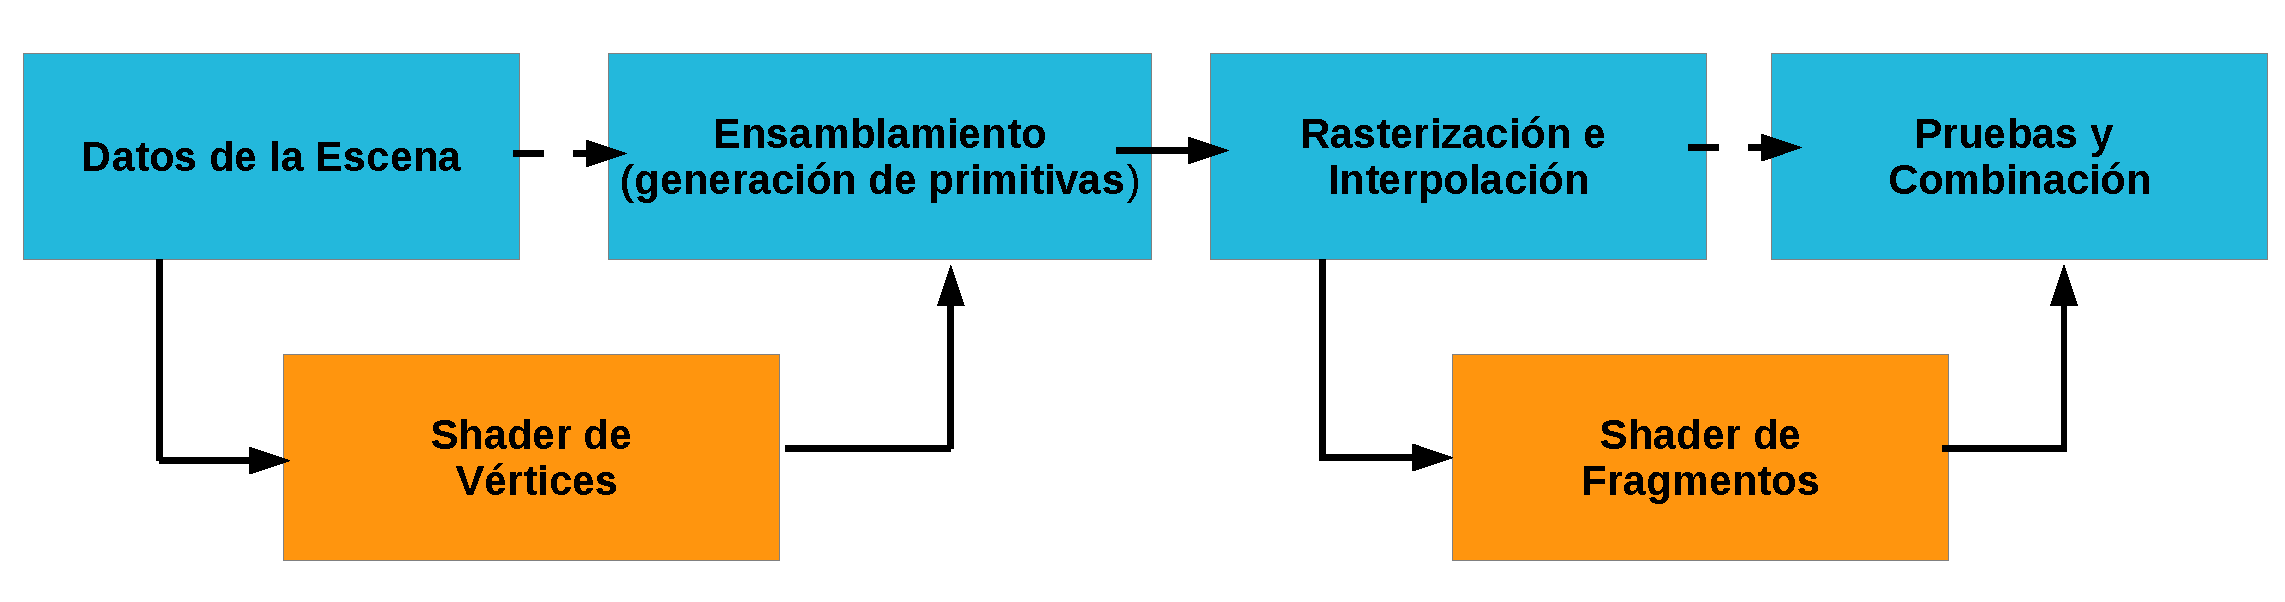
\includegraphics[width=13cm]{figures/pipelinegrafico}
\end{center}
\caption[Pipeline de la GPU con shaders incluidos]{Pipeline de la GPU con shaders incluidos, resaltados en naranja.}
\label{fg:pipelinegrafico}
\end{figure}

Finalizados los cómputos, se vuelcan los resultados en una memoria especial de la GPU, denominada {\em framebuffer}, el cual constituye el dispositivo mediador entre la placa de video y el monitor.
La secuencia explicada constituye el escenario típico de procesamiento de una GPU, excepto en los casos de GPGPU, donde la placa se utiliza para otros propósitos.
De hecho, los resultados de GPGPU no son imágenes, como se explicará más adelante.


\subsection{Características de GLSL}
Presentamos un breve resumen de las principales caracter\'isticas del lenguaje.
Como fue previamente mencionado, existen dos tipos de programas en GLSL, siendo sus nombres {\em Shader de Vértices} y {\em Shader de Fragmentos} respectivamente.
La especificación de las primitivas a dibujar, dentro del pipeline de OpenGL 2.0+, se define por medio de {\em atributos} de vértices y {\em elementos}. 


Los \emph{atributos} son, como su nombre lo indica, atributos o propiedades de un vértice.
El significado se los dará el uso.
Un atributo a considerar consiste en la posición de cada vértice.
Otros atributos comunes están representados por las normales, los colores y las coordenadas de texturas.
Los \emph{elementos} son figuras geométricas (lineas, triángulos, cuadrados) que se forman a partir de unir los vértices definidos por los atributos, ver Fig.~\ref{fg:atributos}.

\begin{figure}[h]
\begin{center}
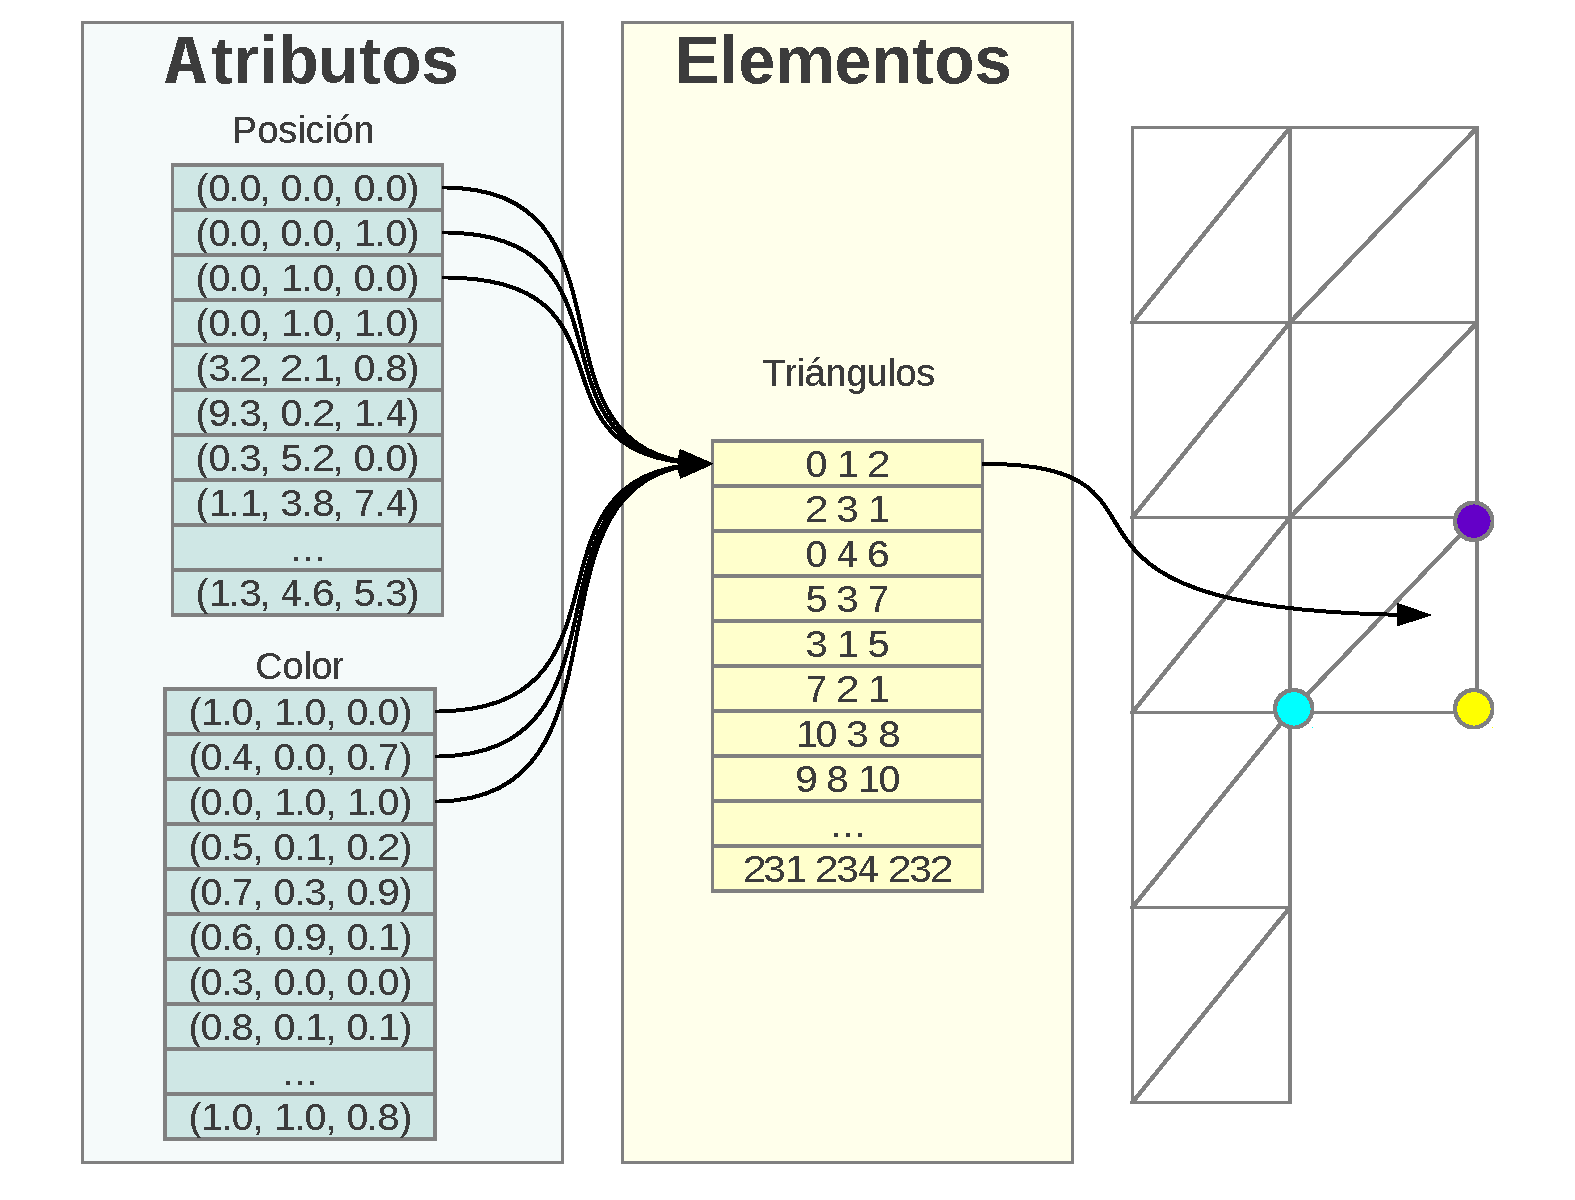
\includegraphics[width=12cm]{figures/atributos}
\end{center}
\caption{Atributos y elementos en GLSL.}
\label{fg:atributos}
\end{figure}

Como fue previamente explicado, la funci\'on del shader de vértices es transformar los v\'ertices de la escena.
De manera simplificada, este shader recibe como entrada la posici\'on del v\'ertice en la escena, y terminada la ejecuci\'on devolver\'a el v\'ertice con su posici\'on modificada.
Tambi\'en podr\'ia devolver el color y otros valores \'utiles que se puedan necesitar en otros pasos de la secuencia de ejecución.
Estos programas reciben los atributos como entrada, así como otras constantes llamadas \emph{uniformes}, para definir la posición final en espacio de clipping (el sub-espacio, proyectado, que dibujará la GPU) de cada vértice.
Los valores \emph{uniformes} pueden ser por ejemplo las matrices de proyección y del modelo o matrices de transformación de normales.
La Fig.~\ref{fg:vertexshader} muestra un ejemplo de un shader de vértices junto a atributos de ejemplo.
El programa de la figura transforma vértices de manera estándar utilizando las matriz {\em modelviewproj} (modelo, vista, proyección), la cual se provee como dos uniformes desde la CPU (uPMatrix y uMVMatrix, las cuales se multiplican).
Los atributos intervinientes son el color y la posición del vértice.
La imagen muestra además que la variable gl\_Position representa la salida del programa, la cual posee coordenadas en el espacio de clipping (entre $[-1,-1,-1]$ y $[1,1,1]$).

\begin{figure}[h]
\begin{center}
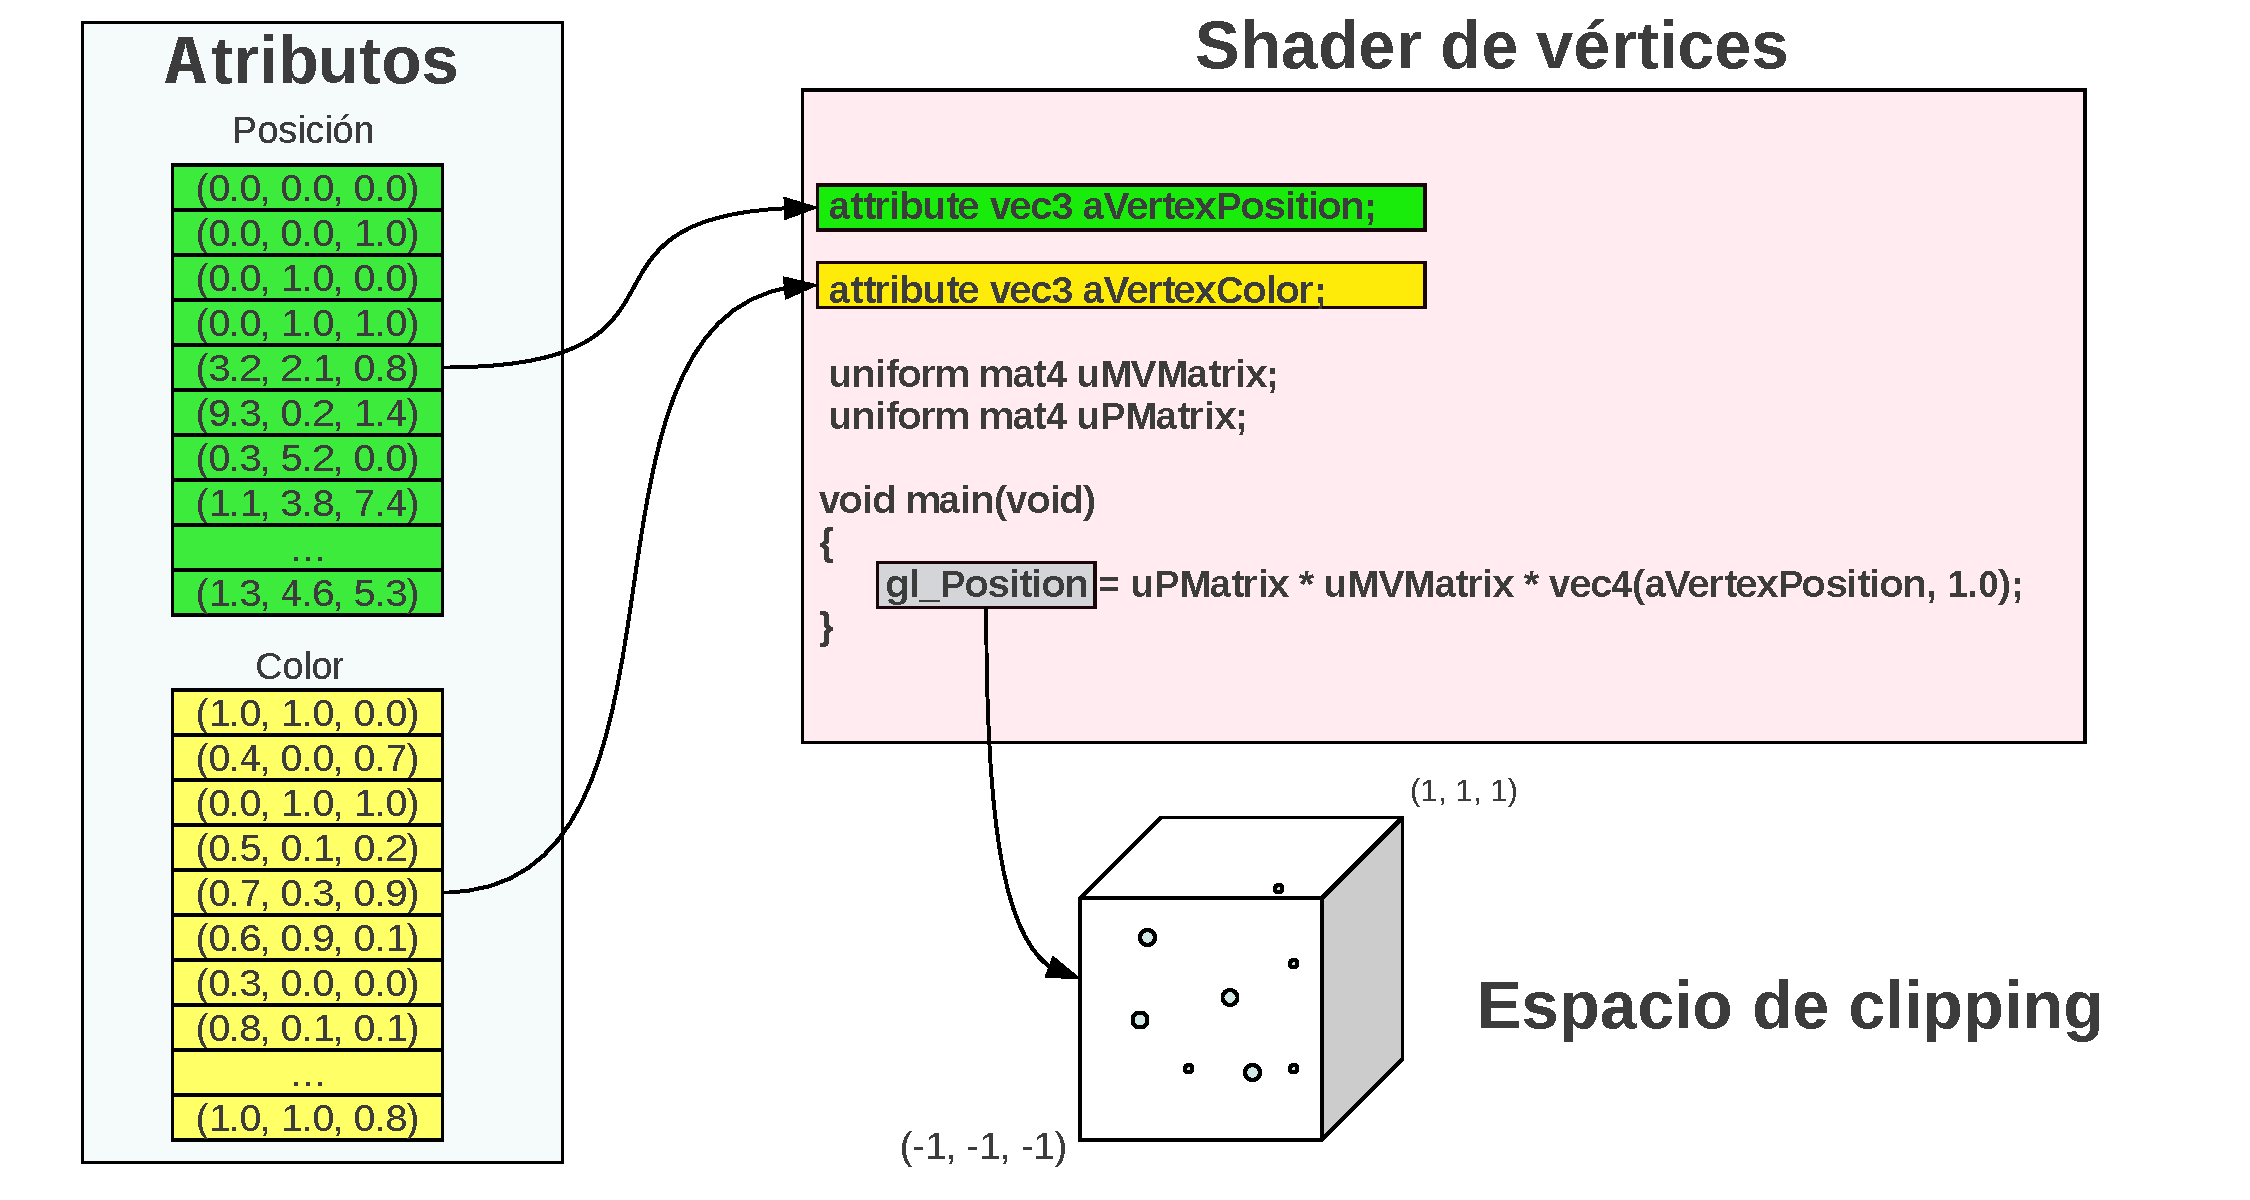
\includegraphics[width=12cm]{figures/vertexshader}
\end{center}
\caption[Atributos y elementos, junto a un ejemplo de shader de vértices en GLSL.]{Atributos y elementos, junto a un ejemplo de shader de vértices en GLSL. Este shader de vértices transforma los vértices en el espacio al espacio del objeto y luego del observador (uMVMatrix). Finalmente realiza una proyección de los mismos sobre el espacio de clipping (uPMatrix).}
\label{fg:vertexshader}
\end{figure}

Una vez que todos los shaders de vértices realizaron sus cómputos, debe procederse a la rasterización, es decir se calcula su posición final en la pantalla a partir de la información del tamaño de la imagen final requerida.
Cada elemento (triángulo, linea, cuadrado) se convierte en una grupo de píxeles (llamado fragmento) que posiblemente se dibujará en la pantalla.
Este proceso puede observarse en la Fig.~\ref{fg:raster}, y a diferencia del shader de vértices, no se permite su programación.


\begin{figure}[h]
\begin{center}
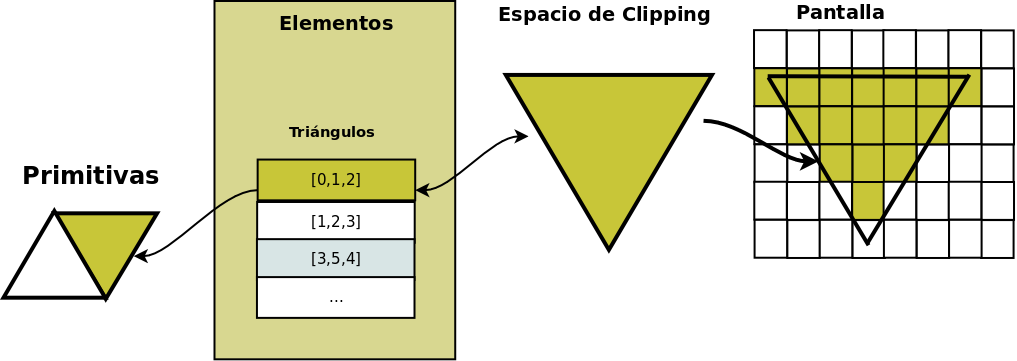
\includegraphics[width=12cm]{figures/raster}
\end{center}
\caption[Proceso de rasterización en la placa gráfica]{Proceso de rasterización en la placa gráfica. En la imagen, un triángulo se convierte en el conjunto de las posiciones de los píxeles que representará en la pantalla.}
\label{fg:raster}
\end{figure}

Finalmente, para calcular el color de cada píxel en pantalla, se utiliza un programa llamado \emph{shader de fragmentos} que calcula el color de cada píxel (o fragmento) que ocupa un elemento (triángulo, linea, cuadrado) individualmente.
Para computar el color final de cada píxel se utilizan \emph{uniformes}, y valores interpolados desde un \emph{shader de vértices}.
Los valores que el programador especifica para ser interpolados se declaran como \emph{varying} en el código de ambos shaders.
La Fig.~\ref{fg:interpolation} muestra un ejemplo de la utilización de un varying para computar el color interpolado de un triángulo.
%La Fig.~\ref{fg:interpolation} muestra el resultado de esta operación.

\begin{figure}[h]
\begin{center}
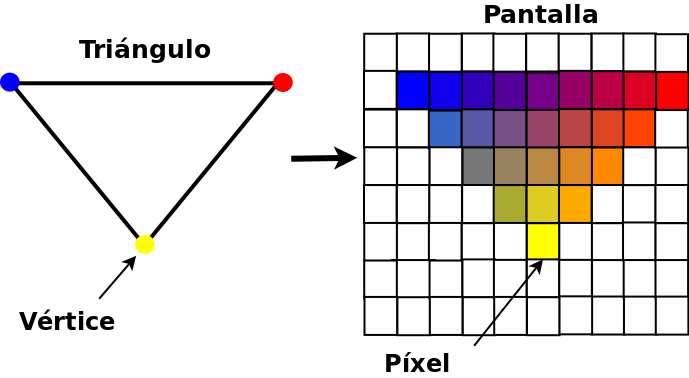
\includegraphics[width=12cm]{figures/interpolation}
\end{center}
\caption[Interpolación automática de colores en la GPU.]{Interpolación automática de colores en la GPU. En la imagen se observan tres vértices de diferente color, junto con el resultado de la rasterización e interpolación de los mismos. Además se muestra un ejemplo de comunicación de datos del shader de vértices al shader de fragmentos. El valor vColor se interpola utilizando la información de los vértices del triángulo, produciendo valores para los fragmentos}
\label{fg:interpolation}
\end{figure}

Similarmente, el shader de fragmentos tiene par\'ametros de entrada y salida.
Generalmente recibe el color interpolado por la etapa previa, pero tambi\'en puede recibir informaci\'on sobre texturas.
A diferencia del shader de vértices, el shader de fragmentos devuelve un único elemento luego de realizar el procesamiento: el {\em color} (excepto en algunos casos específicos, como devolver la profundidad del objeto para cálculo de sombras).
Esta salida representa el color que, de pasar las diversas pruebas, tomar\'a el p\'ixel en pantalla.

\subsection{M\'as sobre el lenguaje}
\paragraph{Integración}
OpenGL incluye desde su versión 2.0 una integración directa con el lenguaje, por lo que es posible programar los distintos shaders de manera transparente, es decir, sin necesidad de compilar o enlazar el código resultante, como sí ocurre en lenguajes rivales como Cg.
Como posible limitación, debe tenerse en cuenta la capacidad de la placa donde se correrá el programa.
Debido a limitaciones de hardware, determinadas placas no permiten bucles en el shader de fragmentos, o tienen un límite en el número de texturas que soportan.
Para agrupar distintas categorías de placas (o capacidades de cómputo), se definieron {\em versiones}.
Las versiones establecen limitaciones a las operaciones en un programa GLSL.
Es as\'i que un código GLSL en una versión determinada debe tener en cuenta las restricciones del mismo.
Sin embargo, la r\'apida evoluci\'on del hardware gr\'afico provoca que las restricciones sean cada vez menores.

\paragraph{Tipos de datos}
Al tener un enfoque gr\'afico, el lenguaje presenta tipos de datos de primer orden diferentes de lenguajes como C. Ejemplo de esto son los {\em vectores} y las {\em matrices}.
GLSL tiene palabras reservadas para estos tipos de datos.
\begin{verbatim}
float f;
int a[4];
float2 v;
mat4 m;
\end{verbatim}
Aqu\'i se definen un flotante (f), un arreglo de cuatro elementos enteros (a), un vector con dos componentes flotantes (v) y una matriz de 16 elementos de tipo flotante (m).
La diferencia entre un arreglo y un vector generalmente responde a la eficiencia.
Otros tipos de datos son los llamados {\em samplers}, los cuales se especifican como {\em uniforms}. Estos representan objetos externos a GLSL, como por ejemplo una textura.
Existen distintos tipos de samplers: {\em sampler1D}, {\em sampler2D} y {\em sampler3D}, representando respectivamente, objetos de una, dos y tres dimensiones. Tambi\'en tipos especiales como {\em samplerCUBE} (utilizado para t\'ecnicas como mapeo de entornos, {\em environment mapping}) y {\em samplerRECT} (permite dimensiones de samplers que no son potencias de dos).

Existe una biblioteca est\'andar que contiene funciones muy \'utiles para el programador. La misma presenta funciones para realizar c\'alculos usuales como m\'aximos, m\'inimos, redondeos, seno, coseno, valores absolutos; y se le suman funciones para el trabajo con vectores, matrices y texturas, como {\em producto escalar}, {\em producto vectorial}, multiplicaci\'on de matrices, multiplicaci\'on de matriz y vector (y viceversa), etc.
El lenguaje utiliza {\em funciones} de la manera usual y con sintaxis similar a C.
Tambi\'en posee una funci\'on {\em principal} que se comporta como {\em main} en C.
La misma se especifica en la aplicaci\'on gr\'afica al crear una instancia de un programa GLSL, la cual entonces representa el punto de entrada al programa.
Se cuenta con estructuras de control usuales, como bucles {\em for} y {\em while}, aunque con determinadas restricciones dependiendo de la versión.
Se presenta a continuaci\'on el cómputo de prop\'osito general en la GPU, GPGPU, el cual difiere de los lenguajes de shader, ya que éstos est\'an dise\~nados para utilizarse \'unicamente con fines gr\'aficos.

\section{GPGPU: CUDA y OpenCL}

\subsection{Introducción}
Como fue discutido, la capacidad de procesamiento de las placas gr\'aficas evolucionó de manera vertiginosa.
La velocidad de transmisi\'on de datos en su memoria interna tambi\'en sufrió una marcada aceleración, superando a memorias tradicionales CPU.
Esto ocurre porque la CPU debe dedicar parte de su poder a control de flujo y {\em cacheo} de datos.
En contraposici\'on, la GPU est\'a dise\~nada para computar en paralelo; se debe aplicar el mismo programa a cada dato (instrucción simple, múltiples datos; Single Instruction, Multiple Data o \acrshort{SIMD}) por lo cual el control de flujo resulta menos necesario.
Debido a estas consideraciones, determinadas compañías decidieron aprovechar la misma como un dispositivo de procesamiento general, más económico que otras soluciones de alto desempeño (por ejemplo, clústers).


Una de las primeras librerías fue desarrollada por la empresa NVIDIA: \acrshort{CUDA} (siglas en ingl\'es de Compute Unified Device Architecture), una arquitectura de computaci\'on paralela de prop\'osito general para placas NVIDIA.
Además, el Khronos Group realizó la primera especificación del estándar abierto OpenCL \cite{Stone2010}.
El mismo representa un intento de apertura de la computación paralela de propósito general (GPGPU), permitiendo implementarse en cualquier procesador.

\subsection{Paradigma de Programación OpenCL}
Deben tenerse en cuenta ciertas consideraciones al implementar algoritmos en OpenCL y CUDA.
En primer lugar, asistimos a un paradigma diferente al usual, ya que el cómputo se realiza en paralelo, a diferencia del computo secuencial tradicional de la máquina de Von Neumann.
Esto implica diversas modificaciones en la forma de programar una solución a un problema dado.
En su versión más simple, un programa secuencial es {\em trivialmente} paralelizable, si el cómputo resulta independiente para cada unidad del programa a ejecutar en cada procesador.
De esta forma, sólo deben verificarse la coherencia de los resultados, en otras palabras, si por ejemplo sumamos dos arreglos, los índices en los arreglos de entrada que se suman se correspondan a los índices correctos en el arreglo de salida.
Para esto, las bibliotecas mencionadas tienen mecanismos de identificación global para cada hilo en ejecución.
Entre los algoritmos trivialmente paralelizables encontramos aquellos que utilizan shaders (cómputos sobre vértices y píxeles independientes), suma de vectores y matrices, etc.

Sin embargo, la programación paralela trae aparejados inconvenientes que fueron resueltos en el paradigma secuencial en el pasado, y parcialmente olvidados por la historia de la computación con el paso de los años.
Entre ellos encontramos a los problemas de concurrencia.
Cuando diferentes procesadores trabajan sobre la misma memoria, deben programarse coherentemente los pasos, garantizando que el resultado sea el esperado.
Los inconvenientes debidos a regiones críticas (elementos de memoria que pueden ser modificados por más de una línea de trabajo) se multiplican en la programación paralela, debido al número de procesos intervinientes.
Surgen además otras dificultades inesperadas.
Por ejemplo, la utilización de condicionales (if), ya que al ejecutar distintas ramas de un if, se produce pérdida de eficiencia.
Esto se debe a las diferencias de velocidad que pueden existir en las ejecuciones de distintas ramas de los condicionales.
Cuando la cantidad de trabajo supera la cantidad de procesadores, los procesos deben terminar al mismo tiempo su cómputo para poder proseguir con el siguiente grupo de procesos.
Esto significa que el proceso más lento del grupo define la velocidad máxima que puede alcanzar el conjunto.
Es por esto que muchas veces la programación debe ser modificada para atender este nuevo objetivo.

Otras limitaciones tienen su causa en el estado actual del hardware gráfico.
Por ejemplo, la recursión aún no se permite en OpenCL, debido al posible consumo de memoria y registros en los procesadores, los cuales aún son limitados.
Debido a la misma causa, otro inconveniente lo constituye la imposibilidad de solicitar memoria de la placa en tiempo de ejecución.
Por todos estos factores, la programación paralela en placas gráficas resulta aún dificultosa.
La elección de implementación de un algoritmo en GPU debe atender a la necesidad de un marcado crecimiento en la velocidad de ejecución del algoritmo en cuestión, y debe ser tomada teniendo en consideración todo lo expuesto aquí.

\subsection{Comparación GPU-CPU}
El paradigma de programación introducido en este apéndice ha demostrado un crecimiento en poder de cómputo prácticamente exponencial.
La Fig.~\ref{fg:cpugpu} muestra curvas con la evolución de las capacidades de cómputo, en número de operaciones flotantes por segundo, de las CPU y las GPU.
Puede observarse que las GPUs superan por mucho el poder computacional de sus CPUs contemporáneas.
Esto debe ser tenido en cuenta en aplicaciones donde los tiempos de cómputo resulten críticos.
Actualmente resulta imposible proveer una implementación de determinadas aplicaciones de tiempo real sin la tecnología GPU, por lo que en la presente tesis se hizo hincapié en esta tecnología.
La implementación del modelo de iluminación DVR del capítulo de renderizado está basada en shaders, donde el cómputo resultó trivialmente paralelizable, resultando en un algoritmo de tiempo real.

\begin{figure}[h]
\begin{center}
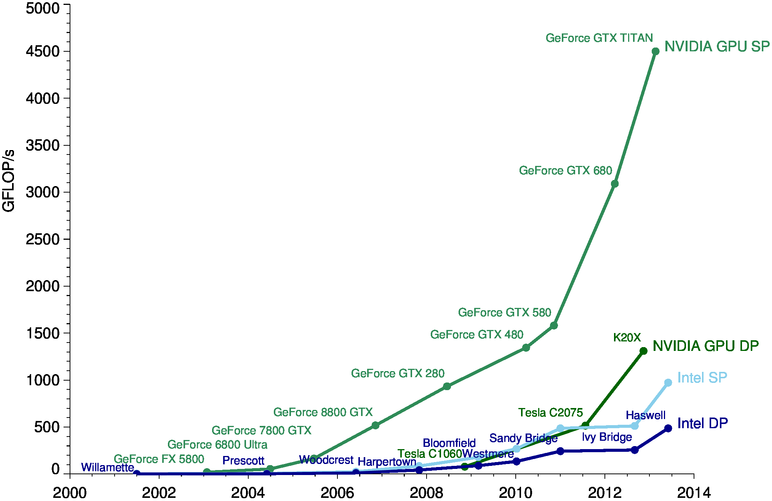
\includegraphics[width=12cm]{figures/cpugpu}
\end{center}
\caption[Comparación de velocidades de cómputo de la CPU y la GPU]{Comparación de velocidades de cómputo de la CPU y la GPU por medio del número de operaciones de punto flotante por segundo (FLOPS, fuente nVidia). La líneas verdes referencian las GPUs.}
\label{fg:cpugpu}
\end{figure}



\subsection{Entorno de programación CUDA}
En esta metodolog\'ia de programaci\'on, existen m\'ultiples hilos (threads) ejecutando en paralelo, ver Fig.~\ref{fg:cuda}.
Los hilos son l\'ogicamente agrupados en {\em bloques} y son enumerados con un \'indice, as\'i hablamos del hilo $i$ de un determinado bloque (también es posible que estén organizados en más de una dimensión).
Los hilos dentro de un bloque se ejecutan en el mismo procesador.
La cantidad de hilos en un bloque queda limitada por los recursos de memoria del procesador de la GPU. Los bloques presentan la misma organizaci\'on, siendo categorizados en {\em grillas}. 
Por lo tanto se habla del bloque $j$ de una determinada grilla.
La memoria total de la GPU se denomina memoria global. Cada hilo tiene su memoria local, s\'olo visible en ese thread.
A su vez, un bloque tiene su memoria local, la cual se comparte por todos los hilos del mismo.
Por \'ultimo, todos los hilos tienen acceso a la memoria {\em global} de la grilla.
Adem\'as, est\'an presentes la memoria de texturas y la memoria constante, las cuales son de s\'olo lectura.
Estas dos y la memoria global se preservan entre llamadas a {\em kernels} (ver siguiente secci\'on).

\begin{figure}[h]
\begin{center}
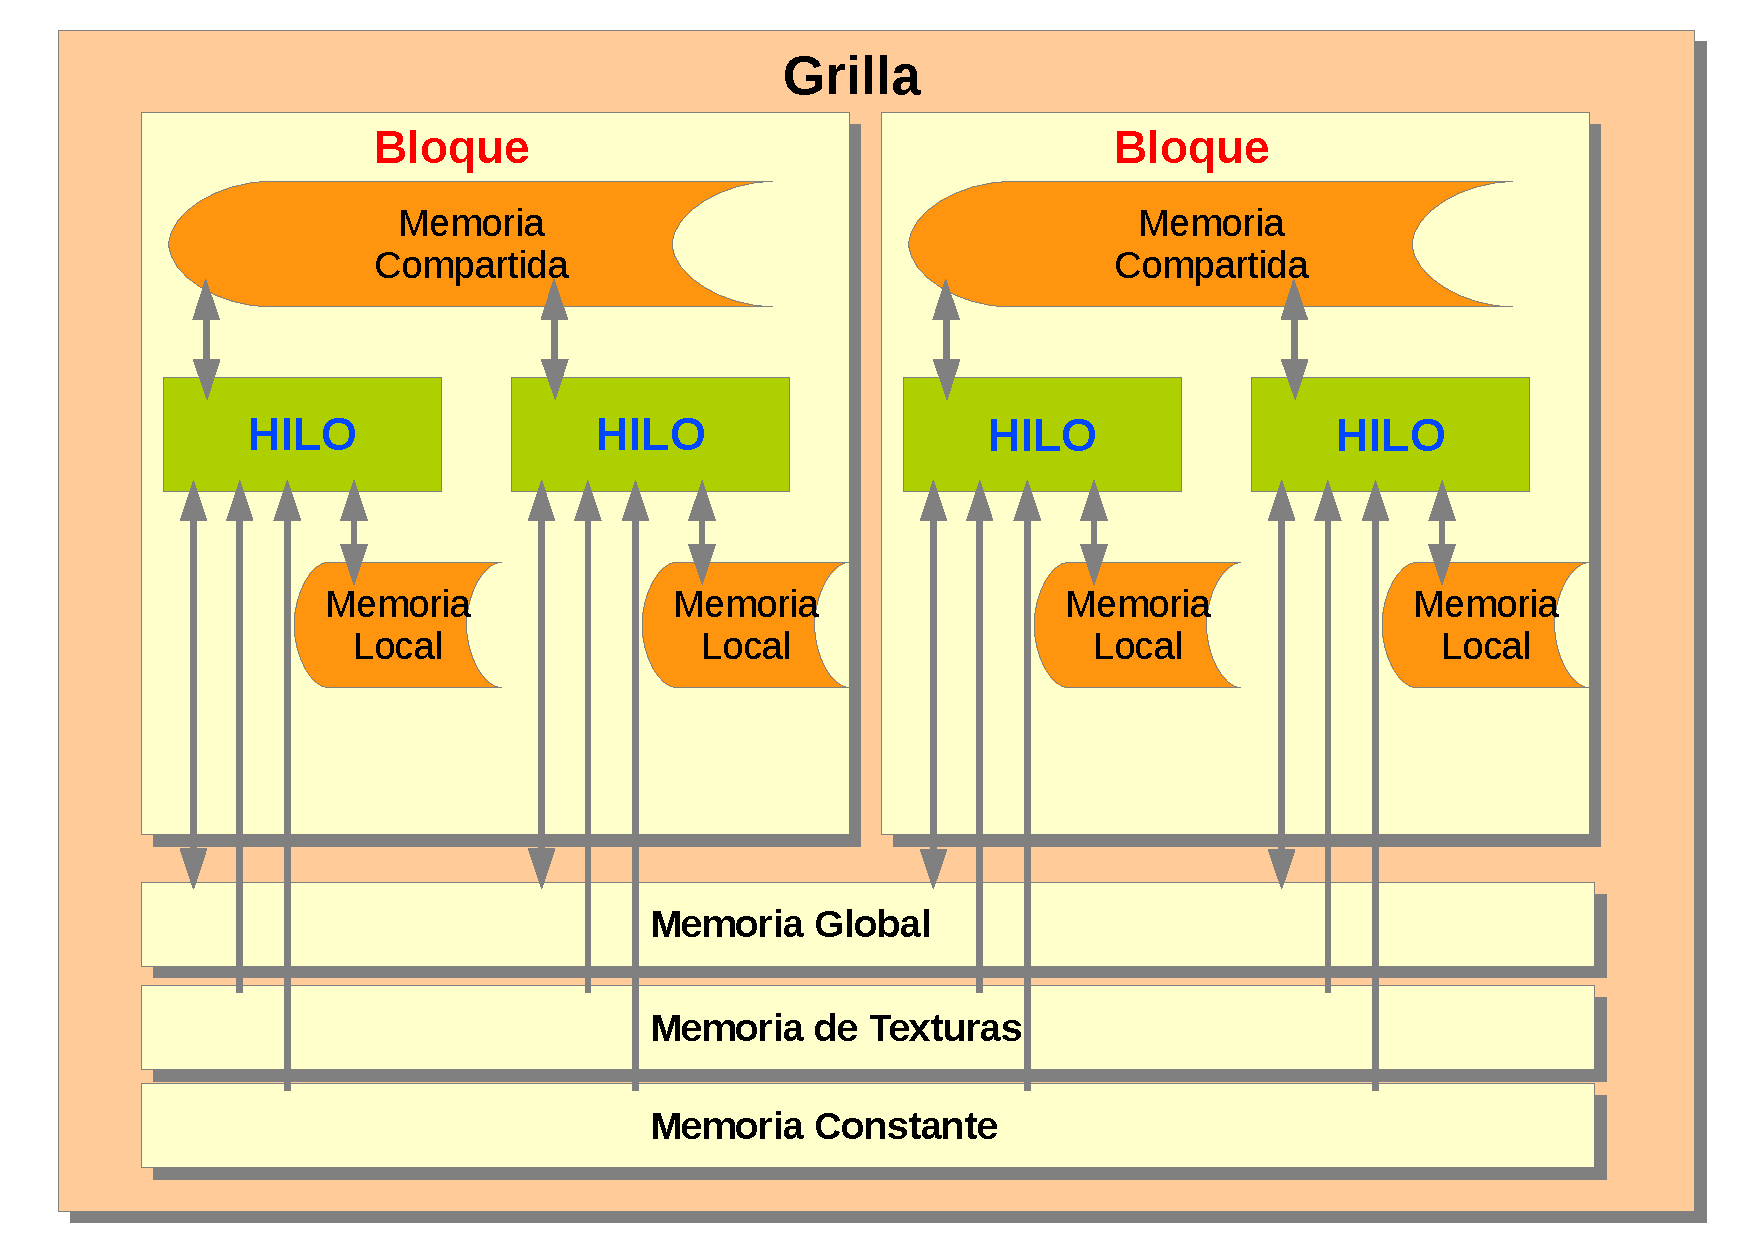
\includegraphics[width=12cm]{figures/cuda}
\end{center}
\caption{Arquitectura CUDA.}
\label{fg:cuda}
\end{figure}


\subsection{Programación en CUDA}
El software que provee CUDA permite a los programadores trabajar en un entorno C o Python (PyCUDA).
En un futuro otros lenguajes como {\em C++} y {\em FORTRAN} tambi\'en ser\'an soportados. 
Existen dos formas de escribir programas CUDA: {\em C para CUDA} y la {\em API del driver de CUDA}.
En el primer caso, se presenta como una extensi\'on a dicho lenguaje junto con un {\em runtime}.
El programador debe escribir funciones a ser ejecutadas en la GPU llamadas {\em kernels}. 
La principal diferencia con una funci\'on C convencional radica en el mecanismo de ejecución, ya que que en lugar de ejecutarse secuencialmente, existen N hilos paralelos ejecutando N instancias de dicha funci\'on. 
El programador debe razonar la solución como varios procesos a ejecutarse en paralelo, los cuales unidos resuelven el problema.
He aqu\'i un ejemplo de un kernel, el cual suma dos vectores:

\begin{verbatim}
__global__ void VecAdd(float* A, float* B, float* C)
{
    int i = threadIdx.x;
    C[i] = A[i] + B[i];
}
\end{verbatim}

\noindent donde \_\_global\_\_ se usa para definir el kernel y denota el car\'acter global del mismo.
La variable reservada threadIdx contiene el ID del thread dentro del bloque que ejecuta la operaci\'on actual, la misma puede tener m\'as de una dimensi\'on, aunque en este caso tiene una sola y por lo tanto se accede al miembro x de la misma.
Para comprender el kernel, debe observarse que cada thread sumar\'a un s\'olo elemento del vector final.
Ejecutar este kernel resulta tan sencillo como una llamada en C, con una salvedad: debe especificarse la cantidad de bloques por grilla (A) y la de hilos por bloque (B), bajo la sintaxis:
$$<<<A , B >>>$$

\begin{verbatim}
int main() {
    int N = 10;
    float* A;
    float* B;
    float* C;
    VecAdd<<<1, N>>>(A, B, C);
}

\end{verbatim}


El driver de CUDA constituye una API de un nivel de abstracci\'on m\'as bajo que el runtime.
De hecho, el runtime est\'a escrito sobre este API.
Su idea principal consiste en utilizar assembler o c\'odigo binario CUDA en la placa, y poder ejecutarlo.
Este c\'odigo se obtiene compilando un kernel.
En este modo tenemos m\'as control sobre lo que ocurre en la GPU, pero tambi\'en resulta m\'as dificultosa la programaci\'on y el {\em debug} del c\'odigo.
Ambos modos proveen m\'etodos para alojar memoria en la GPU, transferirla al CPU, manejar m\'ultiples GPU's, etc.
C para CUDA tiene la opci\'on de emular dispositivos f\'isicos en ausencia de ellos, lo cual puede resultar \'util en caso de no estar los mismos presentes.

\paragraph{NVCC}
CUDA provee un compilador llamado {\em nvcc}.
El mismo se encarga de traducir c\'odigo CUDA a c\'odigo objeto.
Presenta una l\'inea de comandos similar a otros compiladores C como gcc, para facilitar su uso.
Normalmente, un fuente contiene c\'odigo del host (CPU) y del device (GPU) mezclado.
Por lo tanto, el esquema normal de trabajo del compilador consiste en separar c\'odigo a ejecutar en el host del c\'odigo a ejecutar en el device y traducir este \'ultimo hacia assembler ({\em PTX}) o c\'odigo objeto ({\em cubin}).
El c\'odigo del host encontrado en este proceso debe luego ser compilado con un compilador C o bien nvcc puede invocar al mismo y luego producir c\'odigo objeto directamente.

\paragraph{Bibliotecas: cuFFT, cuBLAS}
nVidia ha desarrollado una serie de bibliotecas de uso general para acelerar los cómputos de algoritmos habituales.
La biblioteca cuFFT implementa algoritmos que permiten aplicar la transformada de Fourier directa e inversa a im\'agenes de una o m\'as dimensiones.
Como su nombre lo indica, la biblioteca utiliza el algoritmo {\em fft}, fast fourier transform, útil en aplicaciones de procesamiento de imágenes.
La biblioteca cuBLAS constituye una implementación en GPU de la biblioteca BLAS para cálculos de álgebra lineal.


\subsection{OpenCL}
Dada las similitudes entre CUDA y OpenCL, nos limitaremos aquí a exponer las principales diferencias entre ambas plataformas.
En primer lugar, debe considerarse que, a pesar que la creación de OpenCL está basada en la necesidad de explotación de una placa gráfica, en realidad el diseño de la especificación asume la computación en {\em cualquier} unidad con procesadores.
Es decir que OpenCL también puede ejecutarse en la CPU, por ejemplo.

Debido a esto, los términos equivalentes a aquellos de CUDA, poseen nombres más abstractos.
Cada procesador o placa gráfica que implementa el estándar se denomina {\em dispositivo} o device OpenCL. Cada dispositivo expone una cantidad de {\em unidades de cómputo}, o compute units. Estas unidades de cómputo son grupos de uno o más procesadores.
Los procesadores que forman parte de una unidad de cómputo son llamados {\em elementos
de procesamiento} o processing elements.
Todos los elementos de procesamiento dentro de una misma unidad de cómputo comparten recursos, como memoria y cache.
Esto significa que todos los elementos de procesamiento de una misma unidad de cómputo ejecutan las mismas instrucciones, aunque posiblemente leyendo y escribiendo a lugares diferentes de la memoria. En el caso de expresiones condicionales (if, else) simplemente se desactivan los elementos de procesamiento correspondientes durante la ejecución de la rama condicional que no deben ejecutar.

La memoria en OpenCL se organiza similarmente a la de CUDA, con tres niveles de jerarquía, cada uno con sus tiempos de acceso (global, compartida y privada, en orden descendiente de jerarquía).
El término {\em kernel} refiere al trozo de código a ser ejecutado por una unidad de procesamiento, el cual está escrito en un lenguaje parecido a {\em C}.
Cada kernel será ejecutado en un elemento de procesamiento.
Un conjunto de kernels se agrupa en un grupo de trabajo, el cual se ejecuta en una {\em unidad de cómputo}.
Dado que el código que se escribe resulta el mismo para todos los kernels, la diferenciación entre kernels se lleva a cabo por medio de las función reservada $get\_global\_id(0)$, la cual devuelve el kernel actual dentro de todos los kernels.
Existe un límite a la cantidad de kernels dentro de las unidades de trabajo, pero no a la cantidad de kernels total a ejecutarse.
En caso de que la cantidad total de kernels exceda la capacidad de la GPU, ésta dividirá el trabajo, comenzando a ejecutar algunos grupos de ellos (grupos de trabajo), y una vez terminado esto, ejecutará los siguientes grupos.


La estructura genérica de código python que utiliza OpenCL puede verse a continuación,
donde primero se define un contexto junto a una cola de ejecución, luego se define el programa a partir de un kernel, se lo ejecuta, y se copia el resultado a un arreglo en la CPU.

\begin{verbatim}
Import pyopencl as cl
ctx      = cl.create_some_context()
queue    = cl.CommandQueue(ctx)

# definición programa
prg      = cl.Program(ctx, <kernel_code>).build()

# ejecutar en GPU
prg.main(queue, (N,N), None, <buffers>, <args>) 

# copiar resultado a CPU
cl.enqueue_read_buffer(queue, dest_buf, buf).wait()
\end{verbatim}

donde $kernel\_code$ es un código arbitrario OpenCL.
Un ejemplo de código real OpenCL puede verse a continuación, donde se suman dos arreglos aleatorios $a\_{np}$ y $b\_{np}$. El resultado final se copia al arreglo en CPU $res\_np$ y mostrado por pantalla en la última línea de código.
Los kernels que se ejecutan en la GPU, en paralelo, toman dos arreglos globales de entrada $a\_g$ y $b\_g$, y un arreglo global con el resultado $res\_g$.
El identificador global $gid$ permite diferenciar el kernel ejecutándose, por lo cual el identificador se utiliza como índice en el arreglo resultante, y en los arreglos de entrada, garantizando que las posiciones en el arreglo de entrada y salida son las mismas.
El orden exacto de ejecución corresponde a la GPU, y el programador no debe preocuparse.
Sólo debe tenerse en cuenta la consideración previa, es decir, garantizar la coherencia de los resultados.

\begin{verbatim}
import numpy as np
import pyopencl as cl

a_np = np.random.rand(50000).astype(np.float32)
b_np = np.random.rand(50000).astype(np.float32)

ctx = cl.create_some_context()
queue = cl.CommandQueue(ctx)

mf = cl.mem_flags
a_g = cl.Buffer(ctx, mf.READ_ONLY | mf.COPY_HOST_PTR, hostbuf=a_np)
b_g = cl.Buffer(ctx, mf.READ_ONLY | mf.COPY_HOST_PTR, hostbuf=b_np)

prg = cl.Program(ctx, """
__kernel void sum(__global const float *a_g,
                  __global const float *b_g,
                  __global float *res_g) {
  int gid = get_global_id(0);
  res_g[gid] = a_g[gid] + b_g[gid];
}
""").build()

res_g = cl.Buffer(ctx, mf.WRITE_ONLY, a_np.nbytes)
prg.sum(queue, a_np.shape, None, a_g, b_g, res_g)

res_np = np.empty_like(a_np)
cl.enqueue_copy(queue, res_np, res_g)

# imprimir resultados
print res_np
\end{verbatim}

El identificador $get\_global\_id$ toma un parámetro que indica la cantidad de dimensiones en los que están agrupados los kernels.
Por ejemplo, si trabajáramos con matrices en lugar de arreglos, y decidiéramos multiplicarlas o sumarlas, los identificadores de los kernels podrían estar definidos de a pares.
De esta forma con el par $(get\_global\_id(0), get\_global\_id(1))$, podríamos identificar la fila y columna a la que corresponde el kernel actual, y diseñar nuestro algoritmo para que trabaje solamente sobre un elemento de la matriz actual.

%\section{Aceleración de Algoritmos Fractales en GPU}

%Citar trabajo scipyconar 2014
%\section{Fractales y Multifractales en Computación Gráfica}
\section{Aplicaciones}
Como fue demostrado, además de su utilización en la producción de películas, video juegos, y otras áreas relacionadas a la computación gráfica, la programación de placas gráficas se ha abierto recientemente al cómputo general, por lo que otras ramas de la ciencia han comenzado a utilizar el inmenso poder computacional que proveen.
Este es el caso de física, finanzas, procesamiento de audio y video, astronomía y determinadas ramas de la computación (por ejemplo aprendizaje automatizado, o big data), donde complejas simulaciones tienen lugar en tiempos más acotados gracias a esta nueva herramienta.

En la presente tesis, el poder de la placa gráfica se ha utilizado sobre todo en el cómputo de la aproximación de la ecuación RTE, obteniendo tasas de refresco en tiempo real.
No sólo su utilización fue de gran ayuda, sino que resulta indispensable para cualquier algoritmo gráfico moderno el poder ejecutarse en las mismas si se pretenden alcanzar tiempos interactivos.
Además, se presentó la librería {\em imfractal} en \cite{Baravalle2013}, donde se aceleraron en GPU algunos de los algoritmos útiles para el cómputo de DFs.
Finalmente, se utilizó la GPU para realizar comparaciones en el trabajo presentado en \cite{Baravalle2014_2}

